% section
\section{Image Prediction Architectures} 
 % subsection
 \subsection{LSTM Autoencoder}
  % page 1
  \begin{frame}
   \frametitle{LSTM Autoencoder}
   
   \begin{itemize}
    \item<1-> \glqq Unsupervised Learning of Video Representations using LSTMs\grqq by Srivastava et. al. \cite{Srivastava2015}
    \item<2-> Using the standard LSTM from Hochreiter \& Schmidhuber \cite{Hochreiter1997}
    \item<3-> Autoencoder architecture
    \item<4-> Useful for future image prediction \& image reconstruction
    \item<5-> Typical baseline for newer, more advanced algorithms
   \end{itemize}
   
  \end{frame}
  % page 2
  \begin{frame}
   \frametitle{LSTM Autoencoder}
   
   \begin{figure}[H]
    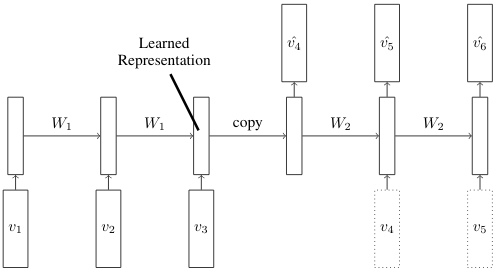
\includegraphics[width=0.7\textwidth]{../Images/srivastava.png}
    \centering
    \caption{Future image prediction model \citep{Srivastava2015}}
    \label{fig:lstm_architecture}
   \end{figure}
  
  \end{frame}
  % page 3
  \begin{frame}
   \frametitle{LSTM Autoencoder}  
  
   \begin{figure}[H]
    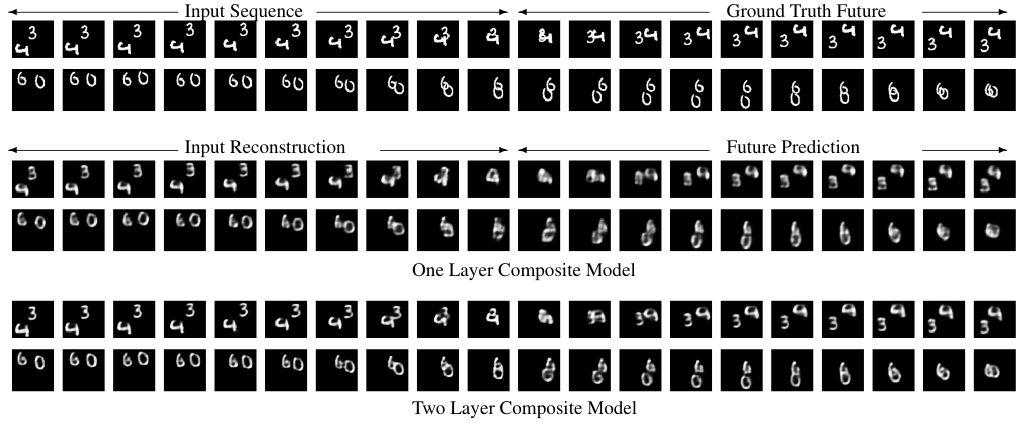
\includegraphics[width=0.7\textwidth]{../Images/srivastava_results_mnist.png}
    \centering
    \caption{Results of MovingMNIST experiment \citep{Srivastava2015}}
    \label{fig:lstm_results_mnist}
   \end{figure}
  
  \end{frame}
 
 % subsection
 \subsection{ConvLSTM Autoencoder}
  % page 1
  \begin{frame}
   \frametitle{ConvLSTM Autoencoder}
   
   \begin{itemize}
    \item<1-> \glqq Convolutional LSTM Network: A Machine Learning Approach for Precipitation Nowcasting\grqq by Shi et. al. \citep{Shi2015}
    \item<2-> Similar to LSTM Autoencoder, but uses ConvLSTM instead
    \item<3-> Outperforms the LSTM Autoencoder
   \end{itemize}
   
  \end{frame}
  % page 2
  \begin{frame}
   \frametitle{ConvLSTM Autoencoder}
   
   \begin{figure}[H]
    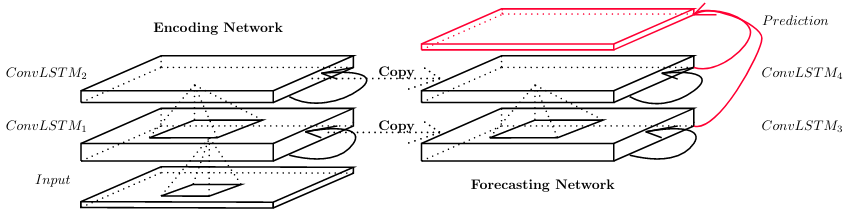
\includegraphics[width=1.0\textwidth]{../Images/shi.png}
    \centering
    \caption{Future image prediction model \citep{Shi2015}}
    \label{fig:convlstm_architecture}
   \end{figure}
  
  \end{frame}
  % page 3
  \begin{frame}
   \frametitle{ConvLSTM Autoencoder}
   
   \begin{figure}[H]
    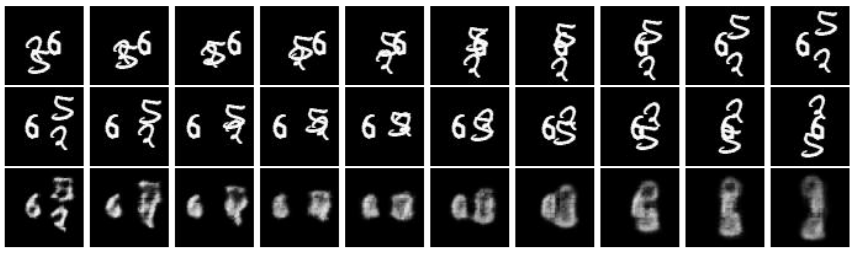
\includegraphics[width=0.7\textwidth]{../Images/shi_results_mnist.png}
    \centering
    \caption{Results of MovingMNIST experiment \citep{Srivastava2015}}
    \label{fig:lstm_architecture}
   \end{figure}  
  
  \end{frame}
 
 % subsection
 \subsection{Spatio-temporal Video Autoencoder}
  % page 1
  \begin{frame}
   \frametitle{Spatio-temporal Video Autoencoder}
   
   \begin{itemize}
    \item<1-> \glqq Spatio-Temporal Video Autoencoder With Differentiable Memory \grqq by Patraucean et. al. \cite{Patraucean2015}
    \item<2->
   \end{itemize}
   
  \end{frame}
  % page 2
  \begin{frame}
   \frametitle{Spatio-temporal Video Autoencoder}
   
   \begin{figure}[H]
    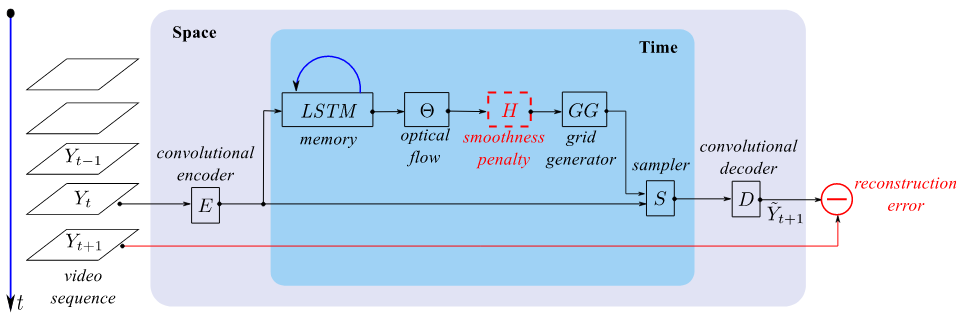
\includegraphics[width=1.0\textwidth]{../Images/patraucean.png}
    \centering
    \caption{Spatio-temporal Video Autoencoder Architecture \citep{Patraucean2015}}
    \label{fig:spatiotemp_architecture}
   \end{figure}
  
  \end{frame}
  % page 3
  \begin{frame}
   \frametitle{Spatio-temporal Video Autoencoder}  
  
   \begin{figure}[H]
    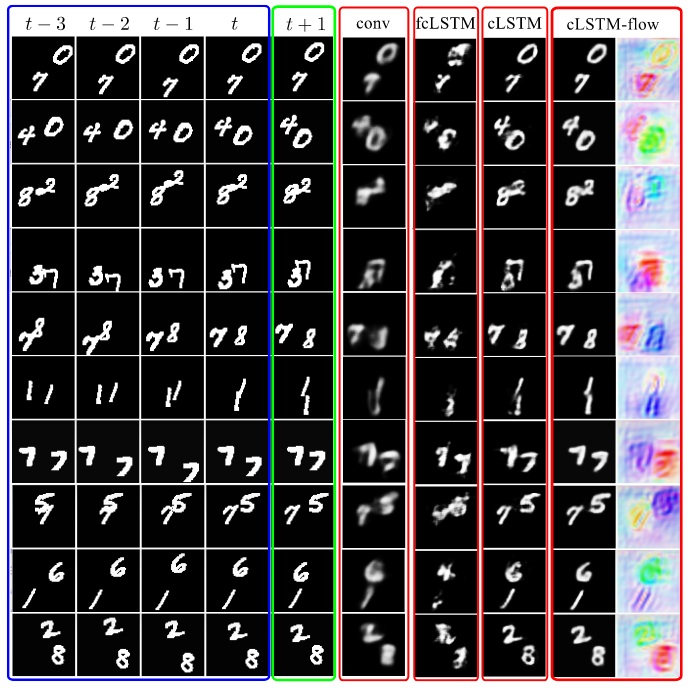
\includegraphics[width=0.55\textwidth]{../Images/patraucean_results_mnist.png}
    \centering
    \caption{Results of MovingMNIST experiment \citep{Patraucean2015}}
    \label{fig:lstm_architecture}
   \end{figure}  
  
  \end{frame}
 
 % subsection
 \subsection{PredNet}
  \begin{frame}
   \frametitle{PredNet}
   
  \end{frame}
  
 % subsection
 \subsection{PredRNN}
  \begin{frame}
   \frametitle{PredRNN}  
  
  \end{frame}
  
 % subsection
 \subsection{PredRNN++}
  \begin{frame}
   \frametitle{PredRNN++}  
  
  \end{frame}